\documentclass[11pt,preprint, authoryear]{elsarticle}

\usepackage{lmodern}
%%%% My spacing
\usepackage{setspace}
\setstretch{1.2}
\DeclareMathSizes{12}{14}{10}{10}

% Wrap around which gives all figures included the [H] command, or places it "here". This can be tedious to code in Rmarkdown.
\usepackage{float}
\let\origfigure\figure
\let\endorigfigure\endfigure
\renewenvironment{figure}[1][2] {
    \expandafter\origfigure\expandafter[H]
} {
    \endorigfigure
}

\let\origtable\table
\let\endorigtable\endtable
\renewenvironment{table}[1][2] {
    \expandafter\origtable\expandafter[H]
} {
    \endorigtable
}


\usepackage{ifxetex,ifluatex}
\usepackage{fixltx2e} % provides \textsubscript
\ifnum 0\ifxetex 1\fi\ifluatex 1\fi=0 % if pdftex
  \usepackage[T1]{fontenc}
  \usepackage[utf8]{inputenc}
\else % if luatex or xelatex
  \ifxetex
    \usepackage{mathspec}
    \usepackage{xltxtra,xunicode}
  \else
    \usepackage{fontspec}
  \fi
  \defaultfontfeatures{Mapping=tex-text,Scale=MatchLowercase}
  \newcommand{\euro}{€}
\fi

\usepackage{amssymb, amsmath, amsthm, amsfonts}

\def\bibsection{\section*{References}} %%% Make "References" appear before bibliography


\usepackage[round]{natbib}

\usepackage{longtable}
\usepackage[margin=2.3cm,bottom=2cm,top=2.5cm, includefoot]{geometry}
\usepackage{fancyhdr}
\usepackage[bottom, hang, flushmargin]{footmisc}
\usepackage{graphicx}
\numberwithin{equation}{section}
\numberwithin{figure}{section}
\numberwithin{table}{section}
\setlength{\parindent}{0cm}
\setlength{\parskip}{1.3ex plus 0.5ex minus 0.3ex}
\usepackage{textcomp}
\renewcommand{\headrulewidth}{0.2pt}
\renewcommand{\footrulewidth}{0.3pt}

\usepackage{array}
\newcolumntype{x}[1]{>{\centering\arraybackslash\hspace{0pt}}p{#1}}

%%%%  Remove the "preprint submitted to" part. Don't worry about this either, it just looks better without it:
\makeatletter
\def\ps@pprintTitle{%
  \let\@oddhead\@empty
  \let\@evenhead\@empty
  \let\@oddfoot\@empty
  \let\@evenfoot\@oddfoot
}
\makeatother

 \def\tightlist{} % This allows for subbullets!

\usepackage{hyperref}
\hypersetup{breaklinks=true,
            bookmarks=true,
            colorlinks=true,
            citecolor=blue,
            urlcolor=blue,
            linkcolor=blue,
            pdfborder={0 0 0}}


% The following packages allow huxtable to work:
\usepackage{siunitx}
\usepackage{multirow}
\usepackage{hhline}
\usepackage{calc}
\usepackage{tabularx}
\usepackage{booktabs}
\usepackage{caption}


\newenvironment{columns}[1][]{}{}

\newenvironment{column}[1]{\begin{minipage}{#1}\ignorespaces}{%
\end{minipage}
\ifhmode\unskip\fi
\aftergroup\useignorespacesandallpars}

\def\useignorespacesandallpars#1\ignorespaces\fi{%
#1\fi\ignorespacesandallpars}

\makeatletter
\def\ignorespacesandallpars{%
  \@ifnextchar\par
    {\expandafter\ignorespacesandallpars\@gobble}%
    {}%
}
\makeatother

\newenvironment{CSLReferences}[2]{%
}

\urlstyle{same}  % don't use monospace font for urls
\setlength{\parindent}{0pt}
\setlength{\parskip}{6pt plus 2pt minus 1pt}
\setlength{\emergencystretch}{3em}  % prevent overfull lines
\setcounter{secnumdepth}{5}

%%% Use protect on footnotes to avoid problems with footnotes in titles
\let\rmarkdownfootnote\footnote%
\def\footnote{\protect\rmarkdownfootnote}
\IfFileExists{upquote.sty}{\usepackage{upquote}}{}

%%% Include extra packages specified by user

%%% Hard setting column skips for reports - this ensures greater consistency and control over the length settings in the document.
%% page layout
%% paragraphs
\setlength{\baselineskip}{12pt plus 0pt minus 0pt}
\setlength{\parskip}{12pt plus 0pt minus 0pt}
\setlength{\parindent}{0pt plus 0pt minus 0pt}
%% floats
\setlength{\floatsep}{12pt plus 0 pt minus 0pt}
\setlength{\textfloatsep}{20pt plus 0pt minus 0pt}
\setlength{\intextsep}{14pt plus 0pt minus 0pt}
\setlength{\dbltextfloatsep}{20pt plus 0pt minus 0pt}
\setlength{\dblfloatsep}{14pt plus 0pt minus 0pt}
%% maths
\setlength{\abovedisplayskip}{12pt plus 0pt minus 0pt}
\setlength{\belowdisplayskip}{12pt plus 0pt minus 0pt}
%% lists
\setlength{\topsep}{10pt plus 0pt minus 0pt}
\setlength{\partopsep}{3pt plus 0pt minus 0pt}
\setlength{\itemsep}{5pt plus 0pt minus 0pt}
\setlength{\labelsep}{8mm plus 0mm minus 0mm}
\setlength{\parsep}{\the\parskip}
\setlength{\listparindent}{\the\parindent}
%% verbatim
\setlength{\fboxsep}{5pt plus 0pt minus 0pt}



\begin{document}



\begin{frontmatter}  %

\title{Question 4}

% Set to FALSE if wanting to remove title (for submission)




\author[Add1]{Peter Meihuizen}
\ead{21831041\sun.ac.za}





\address[Add1]{Stellenbosch University}



\vspace{1cm}





\vspace{0.5cm}

\end{frontmatter}

\setcounter{footnote}{0}



%________________________
% Header and Footers
%%%%%%%%%%%%%%%%%%%%%%%%%%%%%%%%%
\pagestyle{fancy}
\chead{}
\rhead{}
\lfoot{}
\rfoot{\footnotesize Page \thepage}
\lhead{}
%\rfoot{\footnotesize Page \thepage } % "e.g. Page 2"
\cfoot{}

%\setlength\headheight{30pt}
%%%%%%%%%%%%%%%%%%%%%%%%%%%%%%%%%
%________________________

\headsep 35pt % So that header does not go over title




\hypertarget{introduction}{%
\section{\texorpdfstring{Introduction
\label{Introduction}}{Introduction }}\label{introduction}}

Ok so lets see what is popular on netflix.

\hypertarget{analysis}{%
\section{\texorpdfstring{Analysis
\label{Analysis}}{Analysis }}\label{analysis}}

Let's first import the data

We now have a netflix data set showing the information on shows and
movies. This also shows the rating an votes made on IMDB, a well
respected website which gives reliable ratings while accurately
reflecting public opinion towards shows and movies. Therefore I will use
IMDB scores as a metric for quality of a show or movie, and I will use
the number of IMDB votes as a metric for the number of people who
watched the show/movie. To see if the more frequently watched movies are
also highly rated I will plot the 10 most voted movies and there IMDB
scores.

\begin{verbatim}
## # A tibble: 10 x 6
##    title           imdb_votes type  release_year imdb_score production_countries
##    <chr>                <dbl> <chr>        <int>      <dbl> <chr>               
##  1 Inception          2268288 MOVIE         2010        8.8 ['GB', 'US']        
##  2 Forrest Gump       1994599 MOVIE         1994        8.8 ['US']              
##  3 Breaking Bad       1727694 SHOW          2008        9.5 ['US']              
##  4 Django Unchain~    1472668 MOVIE         2012        8.4 ['US']              
##  5 Saving Private~    1346020 MOVIE         1998        8.6 ['US']              
##  6 Stranger Things     989090 SHOW          2016        8.7 ['US']              
##  7 The Walking De~     945125 SHOW          2010        8.2 ['US']              
##  8 Taxi Driver         795222 MOVIE         1976        8.3 ['US']              
##  9 The Imitation ~     748654 MOVIE         2014        8   ['US', 'GB']        
## 10 Full Metal Jac~     723306 MOVIE         1987        8.3 ['GB', 'US']
\end{verbatim}

As can be seen the most voted movies and shows on IMDB all also have
very high ratings. They are also very well\_known movies and tv shows.
This shows that well-known and highly rated movies/shows are the most
popular amongst viewers. It can also be seen that all the top picks are
made by US or GB production companies.

In order to be a successful streaming company, we need people to watch
our content therefore I will use imdb\_votes as the metric for
viewership and see what factors attracts people to watch particular
content. Using the netflix data set, I am going to look at the top 200
shows most viewed shows and movies and see the breakdown of these shows
and movies by genre.

Ok so I want to build a function which shows the distribution of the top
200 shows on netflix. Ok so I'm having issues with my function so I'm
just going to create two data sets each with only movies and only shows
in case I want to see the most popular movie genres also.

Ok now that I have seperated the data sets, we can work out the most
popular 200 shows to see what genres are popular.

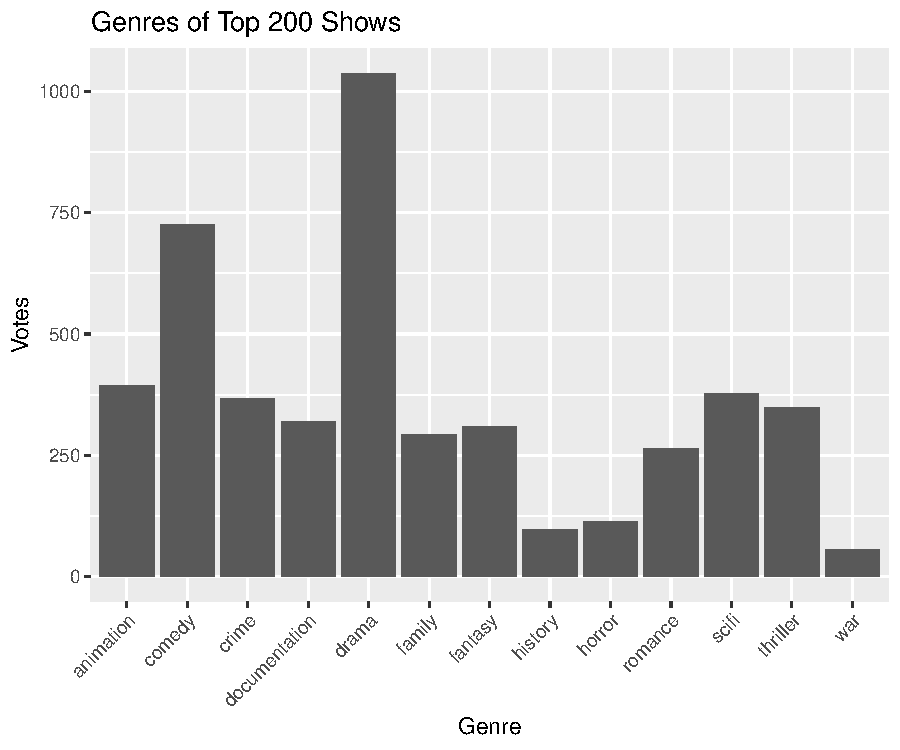
\includegraphics{Question_4_files/figure-latex/unnamed-chunk-4-1.pdf}
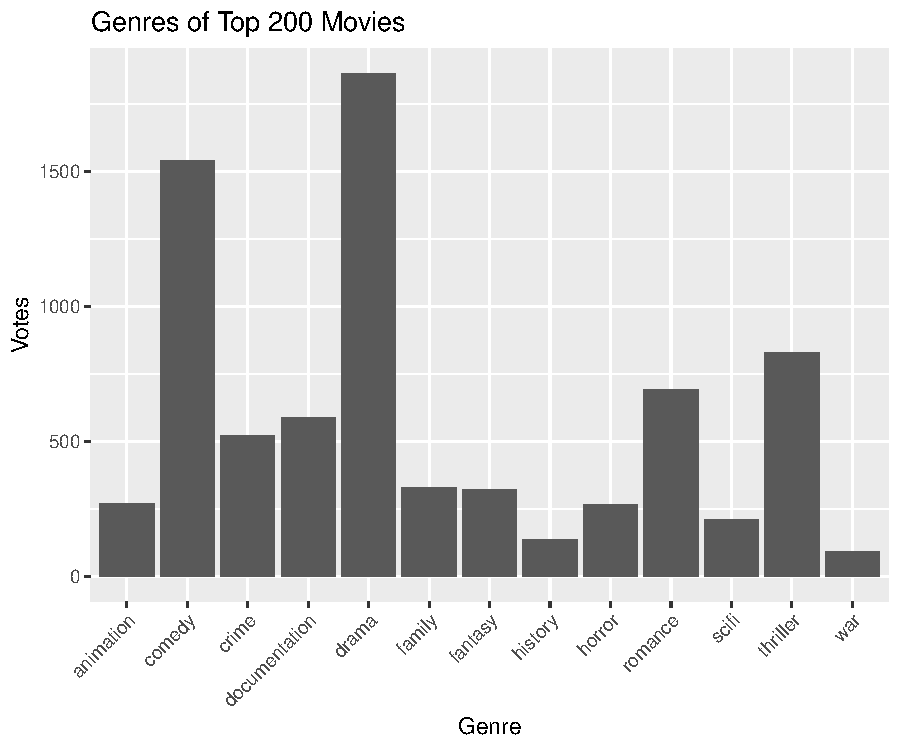
\includegraphics{Question_4_files/figure-latex/unnamed-chunk-4-2.pdf}

Ok so as can be seen by both bargraphs, the top shpws and movies which
are watched are drama and comedy. Drama is the most voted by quite a
long way for both, but comedy also is significantly more popular than
the remaining genres. All of the remaining genres are pretty similar in
popularity. This shows that if you want to make a successful streaming
platform, your content should be predominantly made up of drama shows
and movies, as well as comedies.

\bibliography{Tex/ref}





\end{document}
